\documentclass{beamer}
\usetheme{Warsaw}
\setbeamertemplate{headline}{}

\usepackage{ae,lmodern}
\usepackage[french]{babel}
\usepackage[utf8]{inputenc}
\usepackage[T1]{fontenc}

\usepackage{caption}
\captionsetup[figure]{labelformat=empty}

\PassOptionsToPackage{usenames,dvipsnames}{xcolor}
\usepackage{xcolor,colortbl}
\definecolor{DarkGrey}{HTML}{222222}
\definecolor{DarkBlue}{HTML}{004BA9}
\definecolor{DarkRed}{HTML}{CC1111}
\definecolor{DarkGreen}{HTML}{117711}
\definecolor{DarkOrange}{HTML}{CC7000}
\definecolor{LightGrey}{HTML}{DDDDDD}
\definecolor{LightBlue}{HTML}{F0F8FF}
\definecolor{codegreen}{rgb}{0,0.6,0}
\definecolor{codepurple}{rgb}{0.58,0,0.82}

\usepackage[cache=false]{minted}
\setminted[bash]{
   bgcolor=LightBlue,
   breaklines, breakanywhere,
   frame=single,
   autogobble
}
\usemintedstyle[python]{native}
\setminted[python]{
   bgcolor=black,
   breaklines, breakanywhere,
   autogobble
}

\usepackage{listings}
\usepackage{lstautogobble}
\lstdefinestyle{bash}{
    backgroundcolor=\color{DarkGrey},   
    commentstyle=\color{codegreen},
    keywordstyle=\color{magenta},
    numberstyle=\tiny\color{DarkGrey},
    stringstyle=\color{codepurple},
    basicstyle=\ttfamily\tiny\color{LightGrey},
    escapeinside={\%*}{*)},
    breakatwhitespace=false,         
    breaklines=true,                 
    captionpos=b,                    
    keepspaces=true,                 
    numbers=left,                    
    numbersep=5pt,                  
    showspaces=false,                
    showstringspaces=false,
    showtabs=false,
    showlines=false,
    tabsize=2
}

\usepackage{tikz}
\usetikzlibrary{calc,decorations.pathreplacing,arrows,arrows.meta,shapes,patterns, positioning}
\newcommand\BigLength{14.6em}
\newcommand\Height{2em}
\newcommand\Sep{0.6em}
\newcommand\Center{\BigLength*1/2}
\newcommand\BigBox{\BigLength+\Sep}
\newcommand\HalfBox{\BigLength*1/2-\Sep*1/4}
\newcommand\HalfLength{\BigLength*1/2-\Sep*5/4}
\newcommand\CenterL{\BigLength*1/4-\Sep*1/8}
\newcommand\CenterR{\BigLength*3/4+\Sep*1/8}
\tikzstyle{layer}=[rectangle,thick,text centered,
                     minimum height=\Height,minimum width=\BigLength]
\tikzstyle{short}=[rectangle,thick,text centered,
                     minimum height=\Height,minimum width=\HalfLength]
\tikzstyle{dibox}=[rectangle,thick,semitransparent,
                     minimum height=(\Height+\Sep)*2,minimum width=\BigBox]
\tikzstyle{vmbox}=[rectangle,thick,semitransparent,
                     minimum height=(\Height+\Sep)*3,minimum width=\HalfBox]
\tikzstyle{ctbox}=[rectangle,thick,semitransparent,
                     minimum height=(\Height+\Sep)*2,minimum width=\HalfBox]
\tikzstyle{vebox}=[rectangle,thick,semitransparent,
                     minimum height=(\Height+\Sep)*1,minimum width=\HalfBox]

\usepackage{hyperref}
\usepackage{grffile}


% \AtBeginSection[]
% {
%    \begin{frame}
%       \tableofcontents[currentsection]
%    \end{frame}
% }

% \AtBeginSubsection[]
% {
%    \begin{frame}
%       \tableofcontents[currentsection, currentsubsection, sectionstyle=shaded]
%    \end{frame}
% }

% I added this section
% \AtBeginSubSubsection[]
%     {
%       \begin{frame}
%         \tableofcontents[currentsection,currentsubsection,currentsubsubsection]
%       \end{frame}
%     }

%----------------------------------------------------------------------------------------
\title{Introduction to Data Science}
\subtitle{with Python}
%----------------------------------------------------------------------------------------
\author{Alexis Bogroff}
\date{\today}



\newlength\myheight
\newlength\mydepth
\settototalheight\myheight{Xygp}
\settodepth\mydepth{Xygp}
\setlength\fboxsep{0pt}
\newcommand*\inlinegraphics[1]{%
  \settototalheight\myheight{Xygp}%
  \settodepth\mydepth{Xygp}%
  \raisebox{-\mydepth}{\includegraphics[height=\myheight]{#1}}%
}

\begin{document}


\begin{frame}
   \titlepage
\end{frame}

\begin{frame}\frametitle{Presenter}
   \begin{minipage}{0.3\linewidth}
      \centering
      
\includegraphics[width=0.6\textwidth]{images/AlexisBogroff.png} \\
   \end{minipage}
   \begin{minipage}{0.6\linewidth}
      \noindent Alexis Bogroff \\
      Enseignant data science \\
      à Paris 1 Panthéon-Sorbonne, ESILV, Albert School, UPEC, EM-Lyon, Openclassrooms
   \end{minipage}
   \\[2ex]
   \visible<2->{\begin{itemize}
      \item 6 ans d'enseignement en Data Science et programmation
      \item 2 ans en dev. d'automatisations et pipelines de données
   \end{itemize}}
   \hfill
\end{frame}


\begin{frame}
   \tableofcontents
\end{frame}

% =============================================================================
% =============================================================================
\section{Introduction}
% 3 Hours course
% =============================================================================
% =============================================================================


%------------------------------------------------------------------------------
\subsection{Pourquoi ce cours}
%------------------------------------------------------------------------------
\begin{frame}\frametitle{Pourquoi ce cours}
   \begin{itemize}
      % \item TODO: find article about current enormous investments made to collect and work on data visualization
      % \item TODO: find article about jobs using data
      \item Vous travaillez déjà dans un environnement riche en données
      \item Bénéficiez d'une montée en compétences en visualisation  \inlinegraphics{images/illustrations/up_arrow_green.png}
      \item Citizen Data Scientist: \href{https://www.forbes.fr/business/les-citizen-data-scientists-donner-des-competences-techniques-aux-experts-metier/}{source}
   \end{itemize}
   \begin{figure}[H]
      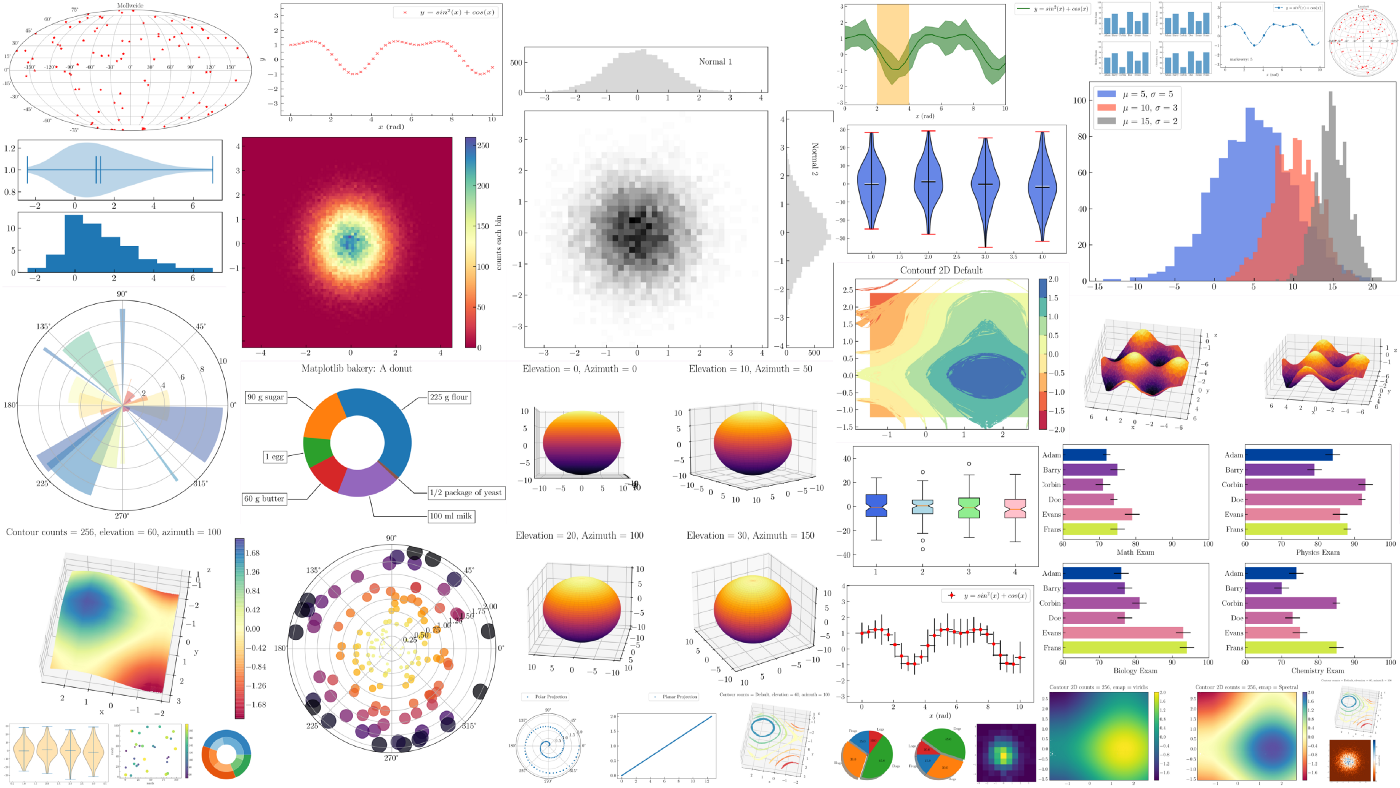
\includegraphics[width=10cm]{images/illustrations/viz_cheat_sheet.png}
   \end{figure}
\end{frame}

\begin{frame}\frametitle{Pourquoi ce cours}
   \begin{itemize}
      \item Formation accélérée : 1 journée, 7h \inlinegraphics{images/illustrations/run.jpeg}
      \item Objectifs
      \begin{itemize}
         \item Revoir et approfondir le choix du type de graphique
         \item Découvrir de nouvelles visualisations
         \item Découvrir comment les implémenter en python
         \item Comprendre les liens entre les différentes librairies Python
      \end{itemize}
   \end{itemize}
\end{frame}


% Reformuler
\begin{frame}\frametitle{Qu'est-ce que la \textit{data viz}}
   \begin{itemize}
      \item Représentation visuelle de la donnée, de l'information
      \item Facilite la vue et la compréhension de tendances (trends), valeurs erronées (outliers), et relations (patterns)
      \item Permet d'expliquer pourquoi ces relations existent, et ce qui pourrait advenir si ces relations persistent
      
      \item Utilise différents types de graphiques: graphiques à barres (bar charts), nuages de points (scatter plots), graphqiues linéaires (line charts), camemberts (pie charts), cartes (maps), etc.
      
      % Formes
      \item Peut être static ou dynamique sur des données historiques, ou bien en temps réel sur un flux continu de nouvelles données
      \item Peut être un graph seul, ou bien un tableau de bord (dashboard)
      \item Peut être intéractif grâce à des systèmes de filtre
      
      \item Permet de représenter des petits volumes de données ou de très larges bases de données (Big Data) sur différents outils
      \item Permet de vulgariser des concepts, et d'atteindre une audience non technique
      \item Permet de prendre des décisions stratégiques
      \item Permet de comprendre des informations utiles de manière intuitive provenant de jeux de données complexes

      \item Des visualisations sont utilisées de manière courantes dans nos vies quotidiennes (charge d'une batterie de smartphone, compteurs de voiture, etc.)
      \item Les bonnes visualisations sont le résultat d'une bonne communication, d'une bonne analyse, et d'un bon design.
      
   \end{itemize}
\end{frame}

% TODO add graphs to show
\begin{frame}\frametitle{Dans quels domaines}
   \begin{itemize}
      \item Marketing
      \item Business
      \item Finance
      \item Industries
      \item Santé
      \item Education
      \item etc.
   \end{itemize}
\end{frame}

\begin{frame}\frametitle{Avantages}
   \begin{itemize}
      \item Rend l'information compréhensible
      \item Peut la rendre plus accessible
      \item Permet une lecture plus rapide
      \item Permet une compréhension plus intuitive
      \item Peut être plus convainquant % (https://blog.reeport.io/fr/les-diagrammes-circulaires-ou-la-data-visualisation-pour-convaincre)
      \item Aide à la prise de décision
   \end{itemize}
\end{frame}

\begin{frame}\frametitle{Risques}
   \begin{itemize}
      \item Biais cognitifs dues aux choix des types de graphs, d'échelles, de couleurs, etc.
      \item L'information sous-jacente peut malgré tout être fausse
      \item Corrélation n'est pas causalité
   \end{itemize}
\end{frame}


% % TODO: histoire de la data viz
% \begin{frame}\frametitle{Histoire de la \textit{data viz}}
%    \begin{itemize}
%       \item Origines
%          \item Source: \href{https://www.perceptualedge.com/articles/Whitepapers/Data_Visualization.pdf}{IBM Cognos Innovation Center}
%    \end{itemize}
% \end{frame}


% % TODO: ajouter chiffres
% \begin{frame}\frametitle{La \textit{data visualization} en chiffres}
%    \begin{itemize}
%       \item Enorme marché en constante évolution %(hors et y compris python - mais aussi outils BI classiques), évolution récente
%       \begin{itemize}
%           \item
%       \end{itemize}
%    \end{itemize}
% \end{frame}


\begin{frame}\frametitle{Dans quel cadre faire de la \textit{data visualization}}
   \begin{itemize}
         \item Compréhension personnelle lors d'une exploration de données
         \item Rapports d'analyses (équipe, direction, clients)
         \item Tableaux de bords (équipe, direction, clients)
         \item Partout (cf. exemples de la vie courante)
   \end{itemize}
\end{frame}

\begin{frame}\frametitle{Qui peut utiliser les visualisations de données}
   \begin{itemize}
      \item Analystes de données
      \item Experts métier
      \item Managers, dirigeants
      \item Développeurs
      \item Chercheurs
      \item Journalistes
      \item Tout le monde
   \end{itemize}
\end{frame}

% ===================================================
% ===================================================
% TODO resume here
% ===================================================
% ===================================================

% TODO reformuler
\begin{frame}\frametitle{Comment faire de la data visualization, quels outils}
   \begin{itemize}
      \item (quel moyen: simples graphs sur Excel / en programmation, outils de dashboards Power BI / Tableau, outils intégrés à un progiciel)
   \end{itemize}
\end{frame}

% TODO REmplir
\begin{frame}\frametitle{Pourquoi avec Python, pour qui}
   \begin{itemize}
      \item 
   \end{itemize}
\end{frame}

% Reformuler
\begin{frame}\frametitle{Quels types de graphs?}
   \begin{itemize}
      \item différents types de données (séries temporelles - finance, audio, images 2D, 3D, graph networks, text avec word cloud). Chercher l'ensemble des types représentatbles avec des graphs
      \item examples pour les différents types de données (sans le code)
      \item exemples de graphs stylés
   \end{itemize}
\end{frame}


\end{document}
